\documentclass[oneside,a4paper,12pt]{extreport}

% Luận văn sử dụng XeLaTeX để hiển thị tiếng Việt ổn định.
\usepackage{fontspec}
\setmainfont{Times New Roman}
\setsansfont{Arial}
\setmonofont{Consolas}

\usepackage[
  a4paper,
  portrait,
  top=30mm,
  bottom=25mm,
  left=35mm,
  right=20mm,
  headheight=15pt,
  footskip=15mm
]{geometry}
\usepackage{setspace}
\onehalfspacing
\usepackage{indentfirst}
\setlength{\parindent}{1.27cm}
\setlength{\parskip}{0pt}

\usepackage{amsmath,amssymb}
\usepackage{graphicx}
\graphicspath{{./}}
\usepackage{booktabs}
\usepackage{array}
\usepackage{enumitem}
\usepackage{microtype}
\setlength{\emergencystretch}{1.5em}
\usepackage{tikz}
\usetikzlibrary{calc}
\usepackage{eso-pic}
\usepackage{titlesec}
\usepackage{fancyhdr}
\usepackage{xurl}
\usepackage[unicode,hidelinks]{hyperref}
\usepackage[numbers,sort&compress]{natbib}

% Thông tin luận văn. Thay các giá trị còn để trong ngoặc vuông trước khi nộp.
\newcommand{\ThesisAuthor}{NGUYỄN VĂN A}
\newcommand{\StudentID}{[MÃ SỐ HỌC VIÊN]}
\newcommand{\Supervisor}{TS. LÊ VIẾT TUẤN}
\newcommand{\Major}{CÔNG NGHỆ THÔNG TIN}
\newcommand{\MajorCode}{[MÃ NGÀNH]}
\newcommand{\ThesisTitle}{CẢI TIẾN MÔ HÌNH TRUY VẤN ĐIỂM\\PHÂN CẤP CHO BÀI TOÁN ĐẾM\\VÀ ĐỊNH VỊ ĐÁM ĐÔNG}
\newcommand{\ThesisTitleEn}{IMPROVING HIERARCHICAL POINT-QUERY MODELS\\FOR CROWD COUNTING AND LOCALIZATION}
\newcommand{\ThesisYear}{2026}

\renewcommand{\chaptername}{Chương}
\renewcommand{\contentsname}{MỤC LỤC}
\renewcommand{\listfigurename}{DANH MỤC HÌNH}
\renewcommand{\listtablename}{DANH MỤC BẢNG}
\renewcommand{\figurename}{Hình}
\renewcommand{\tablename}{Bảng}
\renewcommand{\bibname}{TÀI LIỆU THAM KHẢO}
\renewcommand{\appendixname}{Phụ lục}

\titleformat{\chapter}[display]
  {\normalfont\bfseries\centering\Large}
  {\MakeUppercase{\chaptername}\ \thechapter}
  {8pt}
  {\MakeUppercase}
\titlespacing*{\chapter}{0pt}{10pt}{24pt}
\titleformat{\section}{\normalfont\bfseries\large}{\thesection}{0.8em}{}
\titleformat{\subsection}{\normalfont\bfseries\normalsize}{\thesubsection}{0.8em}{}

\pagestyle{fancy}
\fancyhf{}
\fancyfoot[C]{\thepage}
\renewcommand{\headrulewidth}{0pt}
\fancypagestyle{plain}{
  \fancyhf{}
  \fancyfoot[C]{\thepage}
  \renewcommand{\headrulewidth}{0pt}
}

\hypersetup{
  pdftitle={Cải tiến mô hình truy vấn điểm phân cấp cho bài toán đếm và định vị đám đông},
  pdfauthor={\ThesisAuthor},
  pdfsubject={Luận văn thạc sĩ Công nghệ thông tin},
  pdfkeywords={crowd counting, crowd localization, PET, APG, IFI}
}

\begin{document}

\newcommand{\CoverOuterFrame}{%
  \AddToShipoutPictureBG*{%
    \begin{tikzpicture}[remember picture,overlay]
      \draw[line width=1.5pt]
        ($(current page.north west)+(20mm,-15mm)$)
        rectangle
        ($(current page.south east)+(-15mm,15mm)$);
    \end{tikzpicture}%
  }%
}

\begin{titlepage}
\CoverOuterFrame
\thispagestyle{empty}

\begin{center}
{\bfseries BỘ GIÁO DỤC VÀ ĐÀO TẠO}\par
{\bfseries TRƯỜNG ĐẠI HỌC MỞ THÀNH PHỐ HỒ CHÍ MINH}\par
\vspace{0.8cm}

\begin{tikzpicture}
  \draw[line width=1pt,rounded corners=3pt] (0,0) rectangle (3.2,3.2);
  \node[align=center,font=\bfseries] at (1.6,1.6) {LOGO\\TRƯỜNG};
\end{tikzpicture}\par
\vspace{0.8cm}

{\bfseries\Large \ThesisAuthor}\par
\vspace{2.0cm}

{\bfseries\LARGE \ThesisTitle}\par
\vspace{1.8cm}

{\bfseries LUẬN VĂN THẠC SĨ}\par
\vspace{0.3cm}
{\bfseries NGÀNH: \Major}\par
{Mã ngành: \MajorCode}\par

\vfill
{\bfseries TP. HỒ CHÍ MINH, NĂM \ThesisYear}
\end{center}
\end{titlepage}

\begin{titlepage}
\CoverOuterFrame
\thispagestyle{empty}
\begin{center}
{\bfseries BỘ GIÁO DỤC VÀ ĐÀO TẠO}\par
{\bfseries TRƯỜNG ĐẠI HỌC MỞ THÀNH PHỐ HỒ CHÍ MINH}\par
\vspace{0.8cm}

\begin{tikzpicture}
  \draw[line width=1pt,rounded corners=3pt] (0,0) rectangle (3.0,3.0);
  \node[align=center,font=\bfseries] at (1.5,1.5) {LOGO\\TRƯỜNG};
\end{tikzpicture}\par
\vspace{0.6cm}

{\bfseries\Large \ThesisAuthor}\par
{Mã số học viên: \StudentID}\par
\vspace{1.5cm}

{\bfseries\LARGE \ThesisTitle}\par
\vspace{1.3cm}

{\bfseries LUẬN VĂN THẠC SĨ}\par
{\bfseries NGÀNH: \Major}\par
{Mã ngành: \MajorCode}\par
\vspace{1.3cm}

\begin{flushright}
\begin{minipage}{0.55\textwidth}
\centering
\textbf{NGƯỜI HƯỚNG DẪN KHOA HỌC}\par
\vspace{0.3cm}
\textbf{\Supervisor}
\end{minipage}
\end{flushright}

\vfill
{\bfseries TP. HỒ CHÍ MINH, NĂM \ThesisYear}
\end{center}
\end{titlepage}


\pagenumbering{roman}
\setcounter{page}{1}

\chapter*{LỜI CAM ĐOAN}
\addcontentsline{toc}{chapter}{LỜI CAM ĐOAN}
Tôi cam đoan nội dung luận văn là kết quả nghiên cứu của bản thân dưới sự hướng dẫn của giảng viên hướng dẫn. Các phương pháp, số liệu và kết quả của công trình khác được trích dẫn rõ nguồn. Những kết quả thực nghiệm của luận văn sẽ được báo cáo kèm cấu hình, hạt giống ngẫu nhiên, phân hoạch dữ liệu và tệp kết quả tương ứng để có thể kiểm tra lại.

\chapter*{LỜI CẢM ƠN}
\addcontentsline{toc}{chapter}{LỜI CẢM ƠN}

Tôi xin trân trọng cảm ơn TS. Lê Viết Tuấn đã định hướng nghiên cứu, góp ý về phương pháp và hỗ trợ tôi trong quá trình thực hiện luận văn. Tôi cũng xin cảm ơn quý thầy cô của Trường Đại học Mở Thành phố Hồ Chí Minh đã cung cấp nền tảng kiến thức và môi trường học tập cần thiết.

Tôi chân thành cảm ơn gia đình, đồng nghiệp và bạn bè đã động viên, chia sẻ và hỗ trợ trong suốt thời gian học tập và nghiên cứu.

\begin{flushright}
TP. Hồ Chí Minh, năm \ThesisYear\\
Học viên\\[1.5cm]
\ThesisAuthor
\end{flushright}


\chapter*{TÓM TẮT}
\addcontentsline{toc}{chapter}{TÓM TẮT}
Luận văn nghiên cứu bài toán đếm đồng thời định vị từng cá thể trong ảnh đám đông từ chú thích điểm. Nghiên cứu lấy Point quEry Transformer (PET) làm mô hình nền và khảo sát cách tăng độ ổn định của biểu diễn cũng như quá trình ghép cặp giữa truy vấn và điểm thật trong các cảnh có mật độ, độ phân giải và tỉ lệ đầu người thay đổi mạnh. Hướng tiếp cận giữ lại hai nhánh truy vấn thưa/đặc và cơ chế phân rã quadtree của PET, sau đó tích hợp tín hiệu Auxiliary Point Guidance, nội suy đặc trưng ngầm theo đường dư đa tỉ lệ và ràng buộc ghép cặp/hồi quy có nhận biết tỉ lệ. Phạm vi đánh giá chính gồm ShanghaiTech Part A, ShanghaiTech Part B, UCF-QNRF và NWPU-Crowd; các chỉ số đếm và định vị được báo cáo dưới một quy trình lựa chọn mô hình có kiểm soát. Chương 1 trình bày bối cảnh, khoảng trống nghiên cứu, mục tiêu, phạm vi và các đóng góp của luận văn.

\noindent\textbf{Từ khóa:} đếm đám đông, định vị đám đông, truy vấn điểm, quadtree, APG, nội suy đặc trưng ngầm.

\chapter*{ABSTRACT}
\addcontentsline{toc}{chapter}{ABSTRACT}
This thesis studies joint crowd counting and individual localization from point annotations. Point quEry Transformer (PET) is adopted as the base model. The research investigates how to stabilize feature representation and query-to-target assignment under large variations in crowd density, image resolution, and head scale. The proposed direction preserves PET's sparse/dense query branches and quadtree decomposition while introducing auxiliary point guidance, residual multi-scale implicit feature interpolation, and scale-aware matching and point regression. The main experimental scope comprises ShanghaiTech Part A, ShanghaiTech Part B, UCF-QNRF, and NWPU-Crowd, with counting and localization evaluated under a controlled model-selection protocol. Chapter 1 establishes the research context, gap, objectives, scope, and contributions.

\noindent\textbf{Keywords:} crowd counting, crowd localization, point query, quadtree, auxiliary point guidance, implicit feature interpolation.

\clearpage
\phantomsection
\addcontentsline{toc}{chapter}{MỤC LỤC}
\tableofcontents

\clearpage
\phantomsection
\addcontentsline{toc}{chapter}{DANH MỤC HÌNH}
\listoffigures

\clearpage
\phantomsection
\addcontentsline{toc}{chapter}{DANH MỤC BẢNG}
\listoftables

\clearpage
\pagenumbering{arabic}
\setcounter{page}{1}

\chapter{GIỚI THIỆU}
\label{chap:introduction}

\section{Bối cảnh và lý do chọn đề tài}

Đếm đám đông từ ảnh là bài toán ước lượng số người xuất hiện trong một cảnh quan sát. Bên cạnh giá trị đếm tổng thể, thông tin vị trí của từng cá thể còn cho phép phân tích sự phân bố không gian, xác định khu vực tập trung và hỗ trợ các hệ thống giám sát an toàn. Bài toán có ý nghĩa thực tiễn trong quản lý sự kiện, điều tiết giao thông hành khách, giám sát không gian công cộng và phân tích hành vi đám đông.

Mặc dù đã đạt được nhiều tiến bộ, đếm và định vị đám đông vẫn là bài toán khó do sự thay đổi lớn về mật độ, phối cảnh, kích thước đối tượng, mức độ che khuất, điều kiện chiếu sáng và độ phân giải ảnh. Trong cùng một ảnh, kích thước biểu kiến của đầu người có thể khác nhau đáng kể giữa vùng gần và vùng xa máy ảnh. Ở khu vực mật độ cao, nhiều cá thể chỉ chiếm một số ít điểm ảnh và bị che khuất phần lớn. Những đặc điểm này làm suy giảm độ chính xác của cả phương pháp phát hiện đối tượng lẫn phương pháp hồi quy mật độ \cite{nguyen2020survey}.

Đếm và định vị có quan hệ chặt chẽ nhưng không hoàn toàn tương đương. Một mô hình có thể ước lượng đúng tổng số người trong khi phân bố đáp ứng sai vị trí; ngược lại, mô hình có thể định vị được phần lớn cá thể nhưng tạo điểm trùng hoặc bỏ sót, dẫn đến sai lệch số đếm. Vì vậy, luận văn tiếp cận bài toán dưới dạng dự đoán trực tiếp tập điểm, trong đó mỗi điểm biểu diễn vị trí của một người và số lượng điểm hợp lệ xác định kết quả đếm.

Các phương pháp dựa trên truy vấn điểm tạo ra một khuôn khổ thống nhất cho hai nhiệm vụ trên. P2PNet dự đoán trực tiếp các điểm ứng viên và sử dụng phép gán Hungarian trong quá trình huấn luyện \cite{song2021p2pnet}. PET phát triển cách tiếp cận này bằng cây tứ phân truy vấn điểm, cho phép tăng số truy vấn tại các vùng có mật độ cao thay vì sử dụng một lưới đồng nhất trên toàn ảnh \cite{liu2023pet}. Trong khi đó, APGCC khai thác các điểm phụ trợ và phép nội suy đặc trưng ẩn để cải thiện quá trình học đặc trưng tại những tọa độ không trùng với lưới đặc trưng \cite{chen2024apgcc}. Sự bổ sung về mặt nguyên lý giữa PET và IFI là cơ sở để luận văn nghiên cứu một phương án tích hợp có kiểm soát, hướng đến việc nâng cao đồng thời độ chính xác đếm và định vị.

\section{Phát biểu bài toán}

Cho ảnh đầu vào $I\in\mathbb{R}^{H\times W\times 3}$ và tập chú thích tâm đầu
\begin{equation}
    Y=\{\mathbf y_i\}_{i=1}^{N},
    \qquad \mathbf y_i=(x_i,y_i),
\end{equation}
trong đó $N$ là số người có trong ảnh và $\mathbf y_i$ là tọa độ tâm đầu của người thứ $i$. Mô hình $f_{\theta}$ dự đoán tập
\begin{equation}
    \widehat{Y}=\{(\widehat{\mathbf y}_j,s_j)\}_{j=1}^{M},
\end{equation}
với $\widehat{\mathbf y}_j$ là tọa độ dự đoán và $s_j$ là độ tin cậy của truy vấn thứ $j$. Khi ngưỡng quyết định $\tau$ được xác lập trước, số người dự đoán được tính bởi
\begin{equation}
    \widehat N=\sum_{j=1}^{M}\mathbb I(s_j\geq\tau).
\end{equation}

Bài toán đặt ra hai yêu cầu đồng thời. Thứ nhất, $\widehat N$ phải gần với $N$, được đánh giá bằng sai số tuyệt đối trung bình (Mean Absolute Error, MAE) và căn bậc hai của sai số bình phương trung bình (Root Mean Squared Error, RMSE). Thứ hai, các điểm dự đoán phải tương ứng đúng với vị trí chú thích, được đánh giá bằng precision, recall và F1 theo một ngưỡng khoảng cách xác định trước. Do số đếm được suy ra trực tiếp từ các truy vấn vượt ngưỡng, độ tin cậy phân loại và độ chính xác tọa độ cần được tối ưu và đánh giá trong cùng một khuôn khổ.

Luận văn lựa chọn PET làm mô hình cơ sở và nghiên cứu hai nhóm cải tiến. Nhóm thứ nhất bổ sung IFI theo cấu trúc đường dư nhằm khai thác đặc trưng tại tọa độ liên tục mà vẫn duy trì biểu diễn ban đầu của truy vấn PET. Nhóm thứ hai đưa thông tin tỉ lệ đối tượng vào chi phí ghép cặp và hàm mất mát hồi quy tọa độ. Mỗi thành phần được đánh giá độc lập trước khi xem xét mô hình kết hợp.

\section{Tổng quan các hướng giải quyết}

\subsection{Hồi quy bản đồ mật độ}

Các phương pháp hồi quy mật độ chuyển chú thích điểm thành bản đồ mật độ liên tục, sau đó lấy tích phân trên toàn ảnh để suy ra số người. MCNN sử dụng ba nhánh tích chập có trường tiếp nhận khác nhau và xây dựng bản đồ mật độ đích bằng nhân Gaussian thích nghi hình học \cite{zhang2016mcnn}. CSRNet kết hợp phần trích xuất đặc trưng của VGG-16 với các lớp tích chập giãn nhằm mở rộng trường tiếp nhận mà không làm giảm thêm độ phân giải không gian \cite{li2018csrnet}.

Bayesian Loss và DM-Count tiếp tục cải thiện cách khai thác chú thích điểm. Bayesian Loss mô hình hóa xác suất đóng góp của từng vị trí ảnh đối với mỗi chú thích và tối ưu kỳ vọng số đếm \cite{ma2019bayesian}. DM-Count sử dụng khoảng cách vận chuyển tối ưu giữa phân phối điểm thật và bản đồ mật độ dự đoán, kết hợp mất mát số đếm và Total Variation \cite{wang2020dmcount}. Các phương pháp này tạo tín hiệu huấn luyện dày và đạt kết quả tốt về số đếm, nhưng tọa độ cá thể không phải là đầu ra trực tiếp.

\subsection{Phát hiện và định vị qua bản đồ}

LSC-CNN chuyển chú thích điểm thành mục tiêu phát hiện có kích thước ước lượng, đồng thời sử dụng kiến trúc đa độ phân giải để dự đoán hộp đầu người \cite{sam2021lsccnn}. TopoCount dự đoán bản đồ khả năng và sử dụng ràng buộc tô-pô để kiểm soát số thành phần liên thông; tọa độ cuối được xác định từ tâm của các thành phần sau bước phân ngưỡng \cite{abousamra2021topocount}. Hai hướng này cung cấp thông tin vị trí, nhưng vẫn phụ thuộc vào kích thước hộp giả định hoặc bước hậu xử lý bản đồ.

\subsection{Dự đoán trực tiếp tập điểm}

P2PNet loại bỏ bản đồ mật độ trung gian bằng cách dự đoán trực tiếp một tập điểm ứng viên, đồng thời thực hiện phân loại người--nền và hồi quy độ lệch tọa độ \cite{song2021p2pnet}. CLTR mô hình hóa định vị đám đông như bài toán dự đoán tập hợp bằng Transformer; hàm mục tiêu K-nearest-neighbor Matching Objective bổ sung cấu trúc lân cận vào chi phí ghép cặp \cite{liang2022cltr}. Các phương pháp này thống nhất dạng biểu diễn giữa chú thích và đầu ra, song chất lượng kết quả phụ thuộc đáng kể vào số lượng truy vấn, phép ghép cặp và hiệu chuẩn độ tin cậy.

PET sử dụng cây tứ phân để phân bổ truy vấn theo nội dung ảnh. Một truy vấn ở vùng đông có thể được phân tách thành bốn truy vấn con, trong khi vùng thưa tiếp tục sử dụng truy vấn ở mức hiện tại \cite{liu2023pet}. Nhờ đó, số lượng và mật độ truy vấn thích nghi với phân bố đám đông. APGCC bổ sung các điểm phụ trợ dương và âm quanh chú thích, đồng thời sử dụng IFI để lấy đặc trưng tại tọa độ tùy ý \cite{chen2024apgcc}. Hai công trình giải quyết những khía cạnh khác nhau của phương pháp dự đoán điểm: PET tập trung vào phân bổ truy vấn, còn APGCC tập trung vào tín hiệu học và biểu diễn đặc trưng tại vị trí liên tục.

\section{Hạn chế của các hướng tiếp cận hiện có}

Từ tổng quan tài liệu, luận văn xác định bốn hạn chế liên quan trực tiếp đến bài toán nghiên cứu.

\begin{enumerate}[label=\arabic*)]
    \item \textbf{Sự không thống nhất giữa biểu diễn huấn luyện và đầu ra định vị.} Bản đồ mật độ thuận lợi cho việc ước lượng tổng số nhưng cần thêm bước xử lý để thu được tọa độ cá thể. Sai số đếm thấp vì vậy không bảo đảm chất lượng định vị cao.

    \item \textbf{Phân bổ truy vấn chưa thích nghi ở nhiều phương pháp dự đoán điểm.} Một lưới truy vấn cố định có thể dư thừa tại vùng thưa nhưng không đủ chi tiết tại vùng đông. PET khắc phục một phần hạn chế này bằng cây tứ phân, tuy nhiên hiệu quả vẫn phụ thuộc vào chất lượng biểu diễn của từng truy vấn \cite{liu2023pet}.

    \item \textbf{Đặc trưng tại tọa độ liên tục chưa được khai thác đầy đủ.} Các điểm cần dự đoán không nhất thiết trùng với vị trí rời rạc trên bản đồ đặc trưng. IFI cung cấp cơ chế nội suy học được tại tọa độ tùy ý \cite{chen2024apgcc}, nhưng việc tích hợp cơ chế này vào PET cần bảo toàn thông tin của biểu diễn truy vấn ban đầu.

    \item \textbf{Sai số tọa độ chưa phản ánh đầy đủ sự thay đổi tỉ lệ.} Cùng một độ lệch theo pixel có thể là nhỏ đối với đầu người kích thước lớn nhưng đáng kể đối với đầu người kích thước nhỏ. Vì vậy, chi phí ghép cặp và hồi quy tọa độ cần xem xét thông tin tỉ lệ cục bộ.
\end{enumerate}

Khoảng trống nghiên cứu được xác định là chưa có đánh giá có hệ thống về việc kết hợp cơ chế phân bổ truy vấn phân cấp của PET với IFI theo đường dư và phép ghép cặp nhận biết tỉ lệ trong cùng một mô hình đếm--định vị. Việc kết hợp này không mặc nhiên bảo đảm cải thiện; hiệu quả của từng thành phần phải được kiểm chứng bằng thí nghiệm loại trừ dưới cùng điều kiện dữ liệu và suy luận.

\section{Mục tiêu và câu hỏi nghiên cứu}

\subsection{Mục tiêu tổng quát}

Mục tiêu của luận văn là xây dựng và đánh giá một phương pháp cải tiến trên nền tảng PET nhằm nâng cao chất lượng đếm và định vị đám đông trong điều kiện mật độ và tỉ lệ đối tượng thay đổi.

\subsection{Mục tiêu cụ thể}

\begin{enumerate}[label=\arabic*)]
    \item Xây dựng mô hình cơ sở dựa trên PET và thiết lập giao thức đánh giá thống nhất cho nhiệm vụ đếm và định vị.
    \item Tích hợp IFI theo cấu trúc đường dư trên các đặc trưng đa tỉ lệ, đồng thời duy trì đường truyền đặc trưng ban đầu của PET.
    \item Xây dựng chi phí ghép cặp và hàm mất mát hồi quy tọa độ có xét đến tỉ lệ đối tượng.
    \item Đánh giá riêng từng thành phần và mô hình kết hợp bằng MAE, RMSE, precision, recall và F1.
    \item Khảo sát khả năng khái quát của phương pháp trên các bộ dữ liệu có phân bố mật độ khác nhau.
\end{enumerate}

Các câu hỏi nghiên cứu được đặt ra như sau:

\begin{description}[style=nextline,leftmargin=1.7cm,labelindent=0cm]
    \item[RQ1.] IFI theo cấu trúc đường dư có cải thiện kết quả của mô hình PET cơ sở hay không?
    \item[RQ2.] Phép ghép cặp và hồi quy tọa độ nhận biết tỉ lệ có tạo ra cải thiện bổ sung hay không?
    \item[RQ3.] Mức cải thiện có được duy trì trên các bộ dữ liệu với mật độ và phối cảnh khác nhau hay không?
    \item[RQ4.] Sự cải thiện về số đếm có đồng thời duy trì hoặc nâng cao chất lượng định vị hay không?
\end{description}

\section{Đối tượng và phạm vi nghiên cứu}

Đối tượng nghiên cứu là mô hình học sâu dự đoán điểm cho bài toán đếm và định vị người trong ảnh tĩnh được chú thích bằng tâm đầu. Trọng tâm kỹ thuật gồm cây tứ phân truy vấn điểm, nội suy đặc trưng ẩn đa tỉ lệ, phép ghép cặp Hungarian và hồi quy tọa độ nhận biết tỉ lệ.

Phạm vi dữ liệu chính gồm ShanghaiTech Part A và ShanghaiTech Part B. UCF-QNRF được sử dụng để khảo sát khả năng khái quát trên cảnh có mật độ cao; NWPU-Crowd được đánh giá trên tập validation chính thức. Luận văn không xem xét bài toán theo dõi qua video, nhận dạng danh tính, ước lượng tư thế hoặc phát hiện hành vi bất thường.

Các thí nghiệm sử dụng cùng kiến trúc nền, quy trình tiền xử lý, phân hoạch dữ liệu và thiết lập suy luận khi so sánh các thành phần. Kết quả công bố của các nghiên cứu liên quan chỉ được dùng để tham khảo khi giao thức đánh giá khác với thiết lập thực nghiệm của luận văn.

\section{Phương pháp nghiên cứu}

Nghiên cứu được thực hiện theo phương pháp thực nghiệm định lượng. Trước hết, mô hình PET cơ sở được tái lập và đánh giá để hình thành mốc so sánh. Tiếp theo, IFI theo đường dư và thành phần nhận biết tỉ lệ được bổ sung lần lượt; mỗi thay đổi tạo thành một thí nghiệm loại trừ độc lập. Cuối cùng, các thành phần có hiệu quả được kết hợp và đánh giá trên nhiều bộ dữ liệu.

Việc lựa chọn mô hình được thực hiện trên tập validation hoặc phần holdout tách từ tập huấn luyện. Ngưỡng độ tin cậy, thời điểm dừng và siêu tham số được xác lập trước khi đánh giá trên tập kiểm tra. Các thí nghiệm chính sử dụng hạt giống ngẫu nhiên cố định và lưu lại cấu hình, trọng số mô hình cùng kết quả theo từng ảnh để bảo đảm khả năng kiểm tra và tái lập.

\section{Đóng góp dự kiến của luận văn}

Các đóng góp của luận văn được xác định như sau:

\begin{enumerate}[label=\arabic*)]
    \item Đề xuất cơ chế tích hợp IFI đa tỉ lệ theo đường dư vào PET nhằm khai thác đặc trưng tại tọa độ liên tục mà không loại bỏ biểu diễn truy vấn ban đầu.
    \item Đề xuất thành phần ghép cặp và hồi quy tọa độ nhận biết tỉ lệ cho bài toán dự đoán điểm trong ảnh đám đông.
    \item Xây dựng quy trình thí nghiệm loại trừ để đánh giá riêng ảnh hưởng của từng thành phần đối với cả số đếm và chất lượng định vị.
    \item Cung cấp kết quả thực nghiệm và phân tích lỗi trên các bộ dữ liệu có mức mật độ khác nhau, qua đó làm rõ điều kiện mà phương pháp phát huy hiệu quả hoặc còn hạn chế.
\end{enumerate}

Các đóng góp trên sẽ được xác nhận bằng kết quả thực nghiệm ở Chương 4. Các thành phần kế thừa, gồm phép ghép cặp Hungarian, cây tứ phân của PET và IFI của APGCC, được trình bày với trích dẫn tương ứng \cite{song2021p2pnet,liu2023pet,chen2024apgcc}.

\section{Bố cục luận văn}

Ngoài phần mở đầu, kết luận và tài liệu tham khảo, luận văn gồm bốn chương. Chương 1 trình bày bối cảnh, bài toán, mục tiêu, phạm vi và đóng góp dự kiến. Chương 2 phân tích các công trình liên quan và xác định khoảng trống nghiên cứu. Chương 3 trình bày phương pháp đề xuất, kiến trúc mô hình và hàm mục tiêu. Chương 4 mô tả thiết lập thực nghiệm, phân tích kết quả, thảo luận hạn chế và rút ra kết luận.

\section{Kết chương}

Chương này đã trình bày bối cảnh và ý nghĩa của bài toán đếm--định vị đám đông, phát biểu bài toán dưới dạng dự đoán tập điểm và phân tích khái quát các hướng tiếp cận hiện có. Trên cơ sở các hạn chế được nhận diện, luận văn xác định mục tiêu nghiên cứu là cải tiến PET bằng IFI theo đường dư và thành phần nhận biết tỉ lệ, đồng thời đánh giá phương pháp trên cả hai phương diện đếm và định vị. Chương tiếp theo trình bày chi tiết các công trình liên quan và cơ sở hình thành phương pháp đề xuất.

\chapter{CÁC CÔNG TRÌNH LIÊN QUAN}
\label{chap:related-work}

\section{Khái quát}

Các phương pháp đếm đám đông dựa trên học sâu có thể được phân loại theo dạng biểu diễn đầu ra thành ba nhóm chính: hồi quy bản đồ mật độ, phát hiện hoặc định vị qua bản đồ, và dự đoán trực tiếp tập điểm. Cách phân loại này phản ánh sự chuyển dịch từ mục tiêu chỉ ước lượng tổng số sang mục tiêu đồng thời xác định vị trí từng cá thể. Mỗi nhóm có ưu điểm riêng về tín hiệu huấn luyện, khả năng xử lý mật độ cao và mức độ diễn giải của đầu ra.

Chương này phân tích các công trình tiêu biểu theo bốn khía cạnh: biểu diễn đầu vào và đầu ra; cơ chế học từ chú thích điểm; phương thức xử lý biến thiên mật độ và tỉ lệ; và những hạn chế liên quan đến mục tiêu đếm--định vị trực tiếp. Trọng tâm của phần tổng quan là tiến trình phát triển từ MCNN, CSRNet đến P2PNet, CLTR, PET và APGCC. Các nghiên cứu được lựa chọn đã được đối chiếu với bản toàn văn, ngoại trừ công trình khảo sát của Nguyen và Ngo được kiểm tra theo thông tin xuất bản chính thức do toàn văn thuộc phạm vi truy cập thuê bao.

\section{Phương pháp hồi quy bản đồ mật độ}

\subsection{MCNN và biểu diễn đa tỉ lệ}

MCNN là một trong những công trình đặt nền tảng cho phương pháp đếm bằng bản đồ mật độ. Từ tập chú thích điểm $Y=\{\mathbf y_i\}_{i=1}^{N}$, bản đồ mật độ đích thường được xây dựng theo
\begin{equation}
    D^{\mathrm{gt}}(\mathbf p)
    =\sum_{i=1}^{N}\mathcal K_{\sigma_i}(\mathbf p-\mathbf y_i),
    \label{eq:density-target}
\end{equation}
trong đó $\mathcal K_{\sigma_i}$ là nhân Gaussian tại vị trí $\mathbf y_i$. Tích phân của $D^{\mathrm{gt}}$ trên toàn miền ảnh bằng số chú thích $N$.

MCNN sử dụng ba nhánh mạng tích chập với kích thước bộ lọc khác nhau để mô hình hóa sự biến thiên kích thước đầu người. Độ lệch chuẩn $\sigma_i$ của nhân Gaussian được xác định thích nghi từ khoảng cách đến các điểm lân cận, qua đó phản ánh mật độ cục bộ và ảnh hưởng của phối cảnh \cite{zhang2016mcnn}. Ưu điểm của phương pháp là không cần hộp bao và tạo được tín hiệu giám sát dày từ chú thích điểm. Tuy nhiên, các mức tỉ lệ được biểu diễn bằng những nhánh rời rạc, làm tăng độ phức tạp kiến trúc; đồng thời, tọa độ cá thể không phải là đầu ra trực tiếp.

\subsection{CSRNet và tích chập giãn}

CSRNet sử dụng phần đầu của VGG-16 để trích xuất đặc trưng và một phần sau gồm các lớp tích chập giãn. Tích chập giãn mở rộng trường tiếp nhận mà không cần thêm phép gộp, nhờ đó duy trì độ phân giải không gian tốt hơn khi ước lượng bản đồ mật độ \cite{li2018csrnet}. So với MCNN, CSRNet có kiến trúc tuyến tính và thuận lợi hơn cho việc học đặc trưng ngữ cảnh trong vùng đông.

CSRNet tập trung tối ưu sai khác giữa bản đồ mật độ dự đoán và bản đồ mật độ đích. Kết quả đếm được tính bằng tổng giá trị trên bản đồ dự đoán. Cách tiếp cận này phù hợp với cảnh có mức che khuất lớn, nhưng chất lượng tọa độ sau khi tìm cực đại hoặc phân ngưỡng còn phụ thuộc vào độ phân giải bản đồ và thuật toán hậu xử lý.

\subsection{Bayesian Loss}

Bayesian Loss thay đổi cách sử dụng chú thích điểm thay vì thay đổi kiến trúc dự đoán. Phương pháp xây dựng xác suất mỗi vị trí ảnh đóng góp vào từng chú thích và tối ưu kỳ vọng số đếm tương ứng \cite{ma2019bayesian}. Cách xây dựng này tránh xem bản đồ Gaussian được tạo thủ công là nhãn duy nhất đúng, qua đó giảm sự phụ thuộc vào lựa chọn độ rộng nhân.

Đóng góp quan trọng của Bayesian Loss là chuyển trọng tâm từ hồi quy từng pixel sang giám sát xác suất tại cấp độ chú thích. Tuy vậy, mô hình vẫn sinh bản đồ mật độ, nên việc thu được tập tọa độ cá thể vẫn cần một bước chuyển đổi bổ sung.

\subsection{DM-Count}

DM-Count xem bản đồ mật độ dự đoán và tập điểm chú thích như hai phân phối có tổng khối lượng tương ứng với số người. Hàm mục tiêu kết hợp ba thành phần: sai số số đếm, khoảng cách vận chuyển tối ưu và Total Variation \cite{wang2020dmcount}. Thành phần vận chuyển tối ưu cung cấp tín hiệu hình học toàn cục, trong khi Total Variation hỗ trợ ổn định quá trình tối ưu khi so sánh hai phân phối.

So với mất mát bình phương trên bản đồ Gaussian, DM-Count sử dụng trực tiếp cấu trúc phân phối của chú thích điểm và giảm phụ thuộc vào tham số nhân. Tuy nhiên, đầu ra vẫn là bản đồ mật độ. Phương pháp vì vậy phù hợp với đánh giá số đếm hơn là định vị điểm theo quy trình đầu-cuối.

\subsection{Nhận xét về nhóm hồi quy mật độ}

Các phương pháp dựa trên mật độ có ưu thế khi đối tượng nhỏ, che khuất nhiều và khó xác định hộp bao. Bản đồ mật độ tạo tín hiệu học dày và cho phép suy ra tổng số bằng phép tích phân. Hạn chế cơ bản là sự khác biệt giữa đầu ra tối ưu và đầu ra định vị: hai bản đồ có tổng bằng nhau vẫn có thể phân bố khối lượng rất khác nhau. Do đó, MAE hoặc RMSE thấp không đủ để kết luận mô hình xác định đúng vị trí từng người.

\section{Phương pháp phát hiện và định vị qua bản đồ}

\subsection{LSC-CNN}

LSC-CNN tiếp cận bài toán dưới dạng phát hiện đầu người. Mô hình sử dụng kiến trúc nhiều cột, điều biến đặc trưng từ trên xuống và các đầu dự đoán ở nhiều độ phân giải. Trong trường hợp chỉ có chú thích điểm, kích thước đầu được ước lượng để xây dựng mục tiêu hộp bao phục vụ huấn luyện \cite{sam2021lsccnn}. Số người được suy ra từ số hộp phát hiện, còn vị trí và kích thước đối tượng được biểu diễn trực tiếp qua hộp bao.

Phương pháp cung cấp thông tin ở cấp độ cá thể phong phú hơn bản đồ mật độ. Tuy nhiên, kích thước hộp không có sẵn trong phần lớn bộ dữ liệu đếm đám đông và phải được ước lượng từ quan hệ lân cận. Sai số của kích thước giả định có thể ảnh hưởng đến quá trình học, đặc biệt tại vùng có phối cảnh mạnh hoặc mật độ rất cao.

\subsection{TopoCount}

TopoCount mô hình hóa định vị đám đông bằng một bản đồ khả năng có cấu trúc tô-pô. Hàm mất mát persistence dựa trên persistent homology điều khiển số mode nổi bật trong từng vùng, nhằm hạn chế hiện tượng nhiều cá thể bị gộp thành một đáp ứng hoặc một cá thể tạo ra nhiều đáp ứng giả \cite{abousamra2021topocount}. Khi suy luận, bản đồ khả năng được phân ngưỡng và tâm của từng thành phần liên thông được lấy làm tọa độ dự đoán.

Khác với thao tác đơn thuần tìm cực đại cục bộ, TopoCount đưa cấu trúc liên thông vào quá trình học. Dù vậy, tọa độ cuối vẫn phụ thuộc vào ngưỡng nhị phân hóa và bước xác định thành phần liên thông. Đây là nguồn biến thiên cần được kiểm soát khi so sánh chất lượng định vị.

\section{Phương pháp dự đoán trực tiếp tập điểm}

\subsection{P2PNet}

P2PNet biểu diễn mỗi người bằng một điểm và dự đoán trực tiếp tập tọa độ từ ảnh. Tại mỗi vị trí trên bản đồ đặc trưng, mô hình tạo một số điểm ứng viên, sau đó dự đoán độ tin cậy người--nền và độ lệch tọa độ. Thuật toán Hungarian xác định phép ghép một-một giữa tập dự đoán và tập chú thích sao cho tổng chi phí là nhỏ nhất \cite{song2021p2pnet}. Các điểm không được ghép được huấn luyện về lớp nền.

Khi suy luận, các điểm có độ tin cậy vượt ngưỡng tạo thành kết quả định vị và số lượng điểm chính là số đếm. Nhờ đó, chú thích, đầu ra và chỉ số định vị được thống nhất trong cùng một biểu diễn. P2PNet cũng giới thiệu density Normalized Average Precision để đánh giá sai số vị trí có xét đến biến thiên kích thước đầu \cite{song2021p2pnet}.

Hạn chế của P2PNet là số điểm ứng viên được tạo theo lưới cố định. Cấu hình đủ dày cho vùng đông có thể gây dư thừa ở vùng thưa, tăng chi phí tính toán và làm phép ghép cặp trở nên mơ hồ khi nhiều điểm ứng viên cùng cạnh tranh cho một chú thích.

\subsection{CLTR}

CLTR mô hình hóa định vị đám đông như bài toán dự đoán tập hợp bằng Transformer. Mạng tích chập tạo bản đồ đặc trưng; Transformer encoder mã hóa ngữ cảnh; Transformer decoder nhận các truy vấn học được và hai đầu ra dự đoán tọa độ cùng độ tin cậy \cite{liang2022cltr}. Trong cấu hình được công bố, mô hình sử dụng 500 truy vấn và ngưỡng độ tin cậy 0,35 khi suy luận.

Để giảm sự mơ hồ của phép ghép cặp trong vùng đông, K-nearest-neighbor Matching Objective bổ sung thông tin khoảng cách đến các điểm lân cận vào chi phí Hungarian \cite{liang2022cltr}. Thành phần này giúp phép ghép phản ánh cấu trúc cục bộ của tập điểm. Tuy nhiên, ngân sách truy vấn vẫn được cố định cho mọi ảnh và không thay đổi theo phân bố mật độ từng vùng.

\subsection{Đặc điểm chung của phương pháp dự đoán điểm}

Ưu điểm quan trọng của phương pháp dự đoán điểm là sự thống nhất giữa dạng chú thích và dạng đầu ra. Sai số phân loại ảnh hưởng trực tiếp đến số đếm, còn sai số hồi quy quyết định chất lượng định vị. Mối liên hệ này cũng tạo ra một yêu cầu đánh giá nghiêm ngặt: cải thiện tọa độ nhưng làm tăng số điểm dương giả vẫn có thể khiến MAE và F1 suy giảm. Vì vậy, các chỉ số đếm và định vị phải được báo cáo đồng thời dưới cùng ngưỡng suy luận.

\section{PET và cơ chế truy vấn điểm phân cấp}

PET phát biểu đếm đám đông như một quá trình truy vấn điểm có khả năng phân rã. Mỗi truy vấn được phân loại để xác định có tương ứng với một người hay không và được hồi quy tọa độ. Bộ phân tách cây tứ phân quyết định một truy vấn có cần chia thành bốn truy vấn con tại vùng mật độ cao hay không \cite{liu2023pet}. Nhờ đó, vùng thưa được xử lý bằng truy vấn thưa, trong khi vùng đông nhận mật độ truy vấn cao hơn.

Kiến trúc tổng thể của PET được trình bày trong Hình~\ref{fig:pet-architecture}. Mạng CNN trích xuất đặc trưng ảnh; Transformer encoder với cửa sổ chữ nhật tăng dần mã hóa ngữ cảnh; cây tứ phân tạo các điểm truy vấn thích nghi; Transformer decoder và đầu dự đoán sinh độ tin cậy cùng tọa độ cuối.

\begin{figure}[htbp]
    \centering
    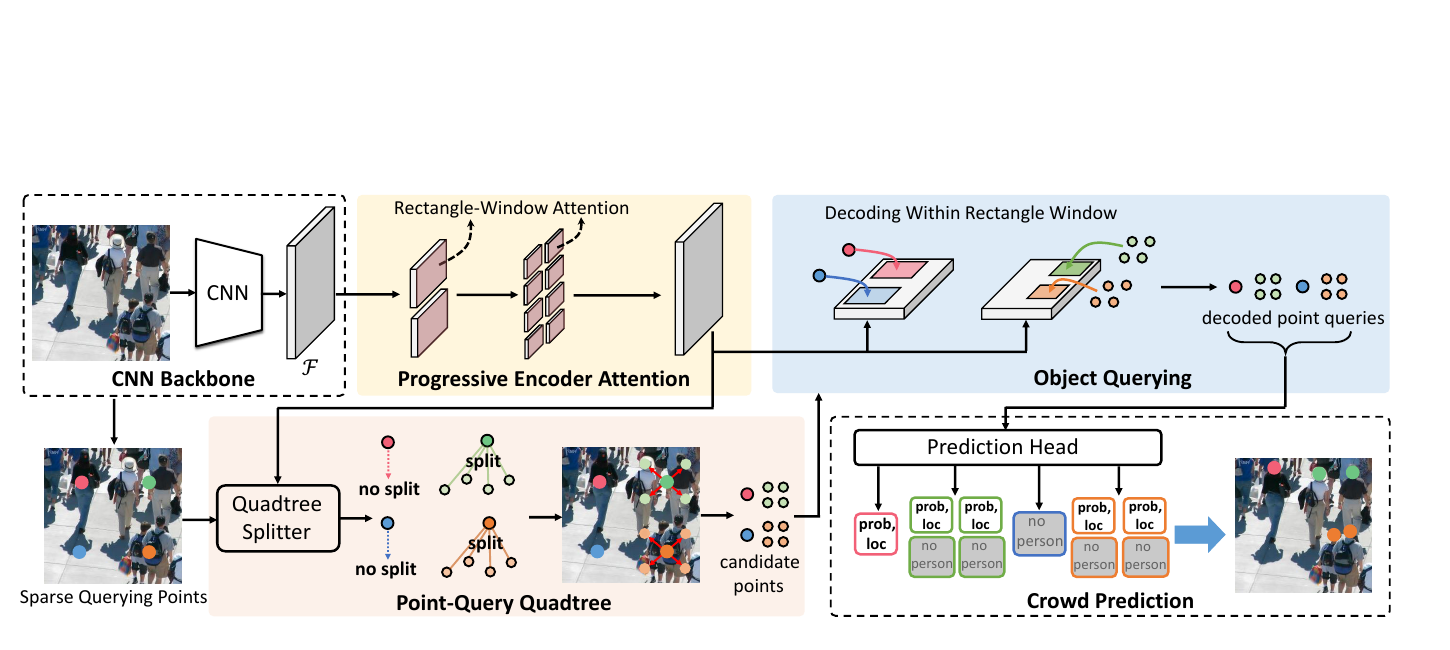
\includegraphics[width=\textwidth]{figures/pet_architecture_source_liu2023.png}
    \caption{Kiến trúc tổng thể của PET. Nguồn: trích từ Hình 2 của Liu và cộng sự \cite{liu2023pet}.}
    \label{fig:pet-architecture}
\end{figure}

PET còn sử dụng progressive rectangle window attention để giới hạn phạm vi tương tác giữa truy vấn và đặc trưng, qua đó giảm chi phí so với attention toàn cục trên ảnh độ phân giải cao. Phụ lục của công trình khảo sát ảnh hưởng của khoảng cách lưới $K$ khi không dùng cây tứ phân trên ShanghaiTech Part A. MAE tương ứng với $K=16,10,8,4$ lần lượt là 62,19; 55,03; 53,59 và 54,16. Kết quả cho thấy việc tăng mật độ truy vấn đến một mức nhất định giúp cải thiện độ chính xác, nhưng lưới quá dày không tiếp tục đem lại lợi ích do sự cạnh tranh giữa các truy vấn tương tự trong phép ghép cặp \cite{liu2023pet}.

PET tạo được sự cân bằng giữa khả năng biểu diễn vùng đông và chi phí tính toán. Tuy nhiên, đặc trưng của truy vấn vẫn gắn với các vị trí rời rạc trên bản đồ đặc trưng; ngoài ra, sai số ghép cặp và hồi quy chưa trực tiếp xét đến sự thay đổi tỉ lệ của đối tượng. Đây là hai khía cạnh được luận văn tiếp tục nghiên cứu.

\section{APGCC và nội suy đặc trưng ẩn}

\subsection{Cơ chế điểm phụ trợ}

APGCC phân tích sự không ổn định của phép ghép giữa điểm dự đoán và điểm chú thích trong quá trình huấn luyện. Với mỗi điểm thật, phương pháp lấy mẫu $k_{\mathrm{pos}}$ điểm phụ trợ dương ở vùng gần và $k_{\mathrm{neg}}$ điểm phụ trợ âm ở vùng xa hơn. Điểm dương được tối ưu với độ tin cậy cao và độ lệch hướng về điểm thật; điểm âm được tối ưu về lớp nền với độ lệch gần bằng không \cite{chen2024apgcc}. Trong cấu hình công bố, $k_{\mathrm{pos}}=k_{\mathrm{neg}}=2$.

Các điểm phụ trợ chỉ được sử dụng để bổ sung tín hiệu giám sát trong giai đoạn huấn luyện; quá trình suy luận vẫn dựa trên các điểm dự đoán chính. Nhờ tạo thêm quan sát quanh chú thích, cơ chế này làm rõ sự khác biệt giữa vùng gần và vùng nền, qua đó cải thiện tính ổn định của quá trình tối ưu \cite{chen2024apgcc}.

\subsection{Implicit Feature Interpolation}

Các điểm phụ trợ có tọa độ liên tục và không nhất thiết trùng với ô trên bản đồ đặc trưng. IFI lấy bốn đặc trưng lân cận $Z_i^*$, độ lệch tương đối $\delta_i^*$ và mã hóa vị trí $\phi(\delta_i^*)$. Một mạng perceptron nhiều lớp $f_\theta$ biến đổi từng bộ thông tin, sau đó các kết quả được tổng hợp theo trọng số diện tích:
\begin{equation}
 F_{\mathrm{IFI}}(x,y)
 =\sum_{i=1}^{4}\frac{S_i}{S}
 f_{\theta}\!\left(Z_i^*,\delta_i^*,\phi(\delta_i^*)\right).
 \label{eq:ifi}
\end{equation}

IFI khác với phép lấy mẫu lân cận gần nhất hoặc nội suy song tuyến tính thuần túy vì hàm nội suy được học và có sử dụng thông tin vị trí tương đối \cite{chen2024apgcc}. Thí nghiệm loại trừ của APGCC so sánh các phương án lấy mẫu khác nhau và cho thấy IFI đầy đủ có đóng góp tích cực trong kiến trúc của công trình này.

Kết quả của APGCC không đồng nghĩa với việc thay thế trực tiếp toàn bộ đặc trưng truy vấn của PET bằng IFI sẽ luôn cải thiện hiệu năng. Luận văn vì vậy xem xét cấu trúc đường dư
\begin{equation}
    \mathbf z
    =\mathbf z_{\mathrm{PET}}
     +\alpha\,\psi(\mathbf z_{\mathrm{IFI}}),
    \label{eq:residual-ifi-concept}
\end{equation}
trong đó $\psi$ là phép biến đổi đặc trưng và $\alpha$ là hệ số điều chỉnh đóng góp của nhánh IFI. Cấu trúc này duy trì đường truyền của đặc trưng PET và cho phép mô hình học dần phần thông tin bổ sung tại tọa độ liên tục. Phương trình~\eqref{eq:residual-ifi-concept} là định hướng thiết kế của luận văn, không phải thành phần nguyên bản của PET hoặc APGCC.

\section{Các nghiên cứu trong bối cảnh Việt Nam}

Nguyen và Ngo công bố một khảo sát về các phương pháp học sâu cho bài toán đếm đám đông trong ảnh đơn. Công trình hệ thống hóa các nhóm phương pháp theo thách thức mà chúng xử lý, bao gồm biến thiên tỉ lệ, phối cảnh, che khuất và nền phức tạp \cite{nguyen2020survey}. Nghiên cứu cung cấp cơ sở tổng quan hữu ích cho việc xác định đặc điểm của bài toán và xu hướng phát triển của phương pháp đếm dựa trên học sâu.

Nguyen và cộng sự xây dựng một hệ thống sử dụng YOLOv3 trên khung hình camera giám sát để phát hiện người, đếm và cảnh báo khu vực tập trung. Nghiên cứu sử dụng 200 ảnh ngoài trời từ STCrowd và SmartCity cùng dữ liệu camera tự thu thập. Các tác giả ghi nhận hạn chế khi người có kích thước nhỏ, ở xa máy ảnh hoặc bị che khuất \cite{nguyen2023yolocrowd}. Phương pháp phù hợp với bối cảnh giám sát có thể quan sát rõ đối tượng, nhưng đầu ra hộp bao và điều kiện mật độ khác với bài toán định vị điểm trong ảnh đám đông rất dày.

Các công trình trên cho thấy nghiên cứu trong nước đã quan tâm cả phương diện tổng quan học thuật và ứng dụng giám sát. Tuy nhiên, trong phạm vi tài liệu được khảo sát, chưa có nghiên cứu đánh giá sự kết hợp giữa truy vấn điểm phân cấp, IFI theo đường dư và hồi quy tọa độ nhận biết tỉ lệ.

\section{So sánh các phương pháp liên quan}

Bảng~\ref{tab:related-methods} tổng hợp dạng đầu ra, cơ chế chính và hạn chế của các phương pháp đối với mục tiêu đếm--định vị trực tiếp. Nhận xét trong cột cuối được giới hạn theo phạm vi bài toán của luận văn và không được hiểu là đánh giá toàn diện chất lượng của từng công trình.

\begin{table}[p]
\centering
\caption{So sánh các phương pháp liên quan theo đầu ra và cơ chế chính}
\label{tab:related-methods}
\begingroup
\small\singlespacing
\setlength{\tabcolsep}{3pt}
\renewcommand{\arraystretch}{1.12}
\begin{tabular}{>{\raggedright\arraybackslash}p{2.25cm}>{\raggedright\arraybackslash}p{2.0cm}>{\raggedright\arraybackslash}p{4.0cm}>{\raggedright\arraybackslash}p{4.35cm}}
\toprule
\textbf{Phương pháp} & \textbf{Đầu ra} & \textbf{Cơ chế chính} & \textbf{Hạn chế đối với bài toán nghiên cứu} \\
\midrule
MCNN \cite{zhang2016mcnn} & Bản đồ mật độ & Ba nhánh CNN; nhân Gaussian thích nghi hình học. & Không trả về tập tọa độ trực tiếp. \\
CSRNet \cite{li2018csrnet} & Bản đồ mật độ & VGG-16 và tích chập giãn. & Tập trung vào mật độ và số đếm. \\
Bayesian Loss \cite{ma2019bayesian} & Bản đồ mật độ & Giám sát kỳ vọng đóng góp tại chú thích. & Cải thiện hàm mất mát nhưng không thay đổi dạng đầu ra. \\
DM-Count \cite{wang2020dmcount} & Bản đồ mật độ & Vận chuyển tối ưu, mất mát số đếm và Total Variation. & Không dự đoán trực tiếp tập tọa độ. \\
LSC-CNN \cite{sam2021lsccnn} & Hộp đầu người & Kích thước giả lập từ chú thích điểm; phát hiện đa độ phân giải. & Phụ thuộc vào chất lượng ước lượng kích thước hộp. \\
\bottomrule
\end{tabular}
\endgroup
\end{table}

\begin{table}[p]
\centering
\caption{So sánh các phương pháp liên quan theo đầu ra và cơ chế chính (tiếp theo)}
\begingroup
\small\singlespacing
\setlength{\tabcolsep}{3pt}
\renewcommand{\arraystretch}{1.12}
\begin{tabular}{>{\raggedright\arraybackslash}p{2.25cm}>{\raggedright\arraybackslash}p{2.0cm}>{\raggedright\arraybackslash}p{4.0cm}>{\raggedright\arraybackslash}p{4.35cm}}
\toprule
\textbf{Phương pháp} & \textbf{Đầu ra} & \textbf{Cơ chế chính} & \textbf{Hạn chế đối với bài toán nghiên cứu} \\
\midrule
TopoCount \cite{abousamra2021topocount} & Bản đồ tô-pô & Persistence loss; phân ngưỡng và thành phần liên thông. & Cần bản đồ trung gian và hậu xử lý để tạo tọa độ. \\
P2PNet \cite{song2021p2pnet} & Tập điểm & Điểm ứng viên và phép ghép Hungarian một-một. & Số điểm ứng viên được phân bổ theo lưới cố định. \\
CLTR \cite{liang2022cltr} & Tập điểm & Transformer và phép ghép có thông tin lân cận. & Ngân sách truy vấn cố định, không thích nghi theo vùng ảnh. \\
PET \cite{liu2023pet} & Tập điểm & Cây tứ phân truy vấn điểm phụ thuộc dữ liệu. & Đặc trưng truy vấn gắn với vị trí rời rạc; chưa xét tỉ lệ trong hồi quy. \\
APGCC \cite{chen2024apgcc} & Tập điểm & Điểm phụ trợ và IFI tại tọa độ liên tục. & Hiệu quả được kiểm chứng trong kiến trúc APGCC, chưa được đánh giá khi tích hợp vào PET. \\
\bottomrule
\end{tabular}
\endgroup
\end{table}

Nhóm hồi quy mật độ thuận lợi cho việc ước lượng tổng số nhưng không cung cấp tập điểm một cách tự nhiên. Nhóm phát hiện hoặc định vị qua bản đồ tạo được thông tin vị trí, song cần kích thước hộp giả định hoặc hậu xử lý. Nhóm dự đoán điểm thống nhất chú thích với đầu ra, nhưng phụ thuộc vào chiến lược phân bổ truy vấn, phép ghép cặp và hiệu chuẩn độ tin cậy. PET giải quyết bài toán phân bổ truy vấn bằng cây tứ phân; APGCC cung cấp cơ chế khai thác đặc trưng tại tọa độ liên tục. Đây là cơ sở lý thuyết để xây dựng phương pháp của luận văn.

\section{Khoảng trống nghiên cứu}

Tổng quan các công trình liên quan cho thấy ba vấn đề còn cần được nghiên cứu. Thứ nhất, PET phân bổ truy vấn thích nghi theo mật độ nhưng đặc trưng tại mỗi truy vấn vẫn chịu ràng buộc của lưới đặc trưng rời rạc. Thứ hai, IFI cho phép lấy đặc trưng ở tọa độ liên tục, nhưng chưa có bằng chứng cho thấy việc tích hợp trực tiếp vào PET sẽ duy trì ổn định biểu diễn và độ tin cậy của mô hình. Thứ ba, phép ghép cặp và hồi quy tọa độ thường dựa trên khoảng cách tuyệt đối, chưa phản ánh đầy đủ sự biến thiên kích thước đầu do phối cảnh.

Từ các khoảng trống trên, luận văn tập trung vào hai thành phần: IFI đa tỉ lệ theo cấu trúc đường dư và phép ghép cặp, hồi quy tọa độ nhận biết tỉ lệ. Phương pháp được đánh giá theo quy trình thí nghiệm loại trừ, trong đó mỗi thành phần chỉ được chấp nhận khi tạo ra cải thiện nhất quán và không làm suy giảm đáng kể chất lượng định vị. Cách đánh giá này giúp phân biệt đóng góp của luận văn với các thành phần đã được công bố trong PET, P2PNet và APGCC.

\section{Kết chương}

Chương này đã phân tích quá trình phát triển của các phương pháp đếm đám đông từ hồi quy bản đồ mật độ đến dự đoán trực tiếp tập điểm. MCNN và CSRNet khai thác đặc trưng đa tỉ lệ trong bản đồ mật độ; Bayesian Loss và DM-Count cải thiện cách học từ chú thích điểm; LSC-CNN và TopoCount bổ sung khả năng định vị qua hộp hoặc bản đồ; P2PNet và CLTR thống nhất đầu ra dưới dạng tập điểm; PET phân bổ truy vấn thích nghi bằng cây tứ phân; APGCC khai thác điểm phụ trợ và nội suy đặc trưng tại tọa độ liên tục. Trên cơ sở đó, luận văn xác định khoảng trống nghiên cứu và hình thành định hướng cải tiến PET bằng IFI theo đường dư kết hợp thông tin tỉ lệ. Chương 3 sẽ trình bày chi tiết kiến trúc và hàm mục tiêu của phương pháp đề xuất.

\chapter{PHƯƠNG PHÁP ĐỀ XUẤT}
\label{chap:method}

% Khung nội dung được đồng bộ với các model_recipe T1--T4 trong repo.
\section{Kiến trúc PET nền}
\section{Baseline APG và ràng buộc tương phản cục bộ}
\section{Nội suy đặc trưng ngầm đa tỉ lệ theo đường dư}
\section{Ghép cặp nhận biết tỉ lệ}
\section{Hồi quy điểm chuẩn hóa theo tỉ lệ}
\section{Count head phụ trợ và điều kiện sử dụng}
\section{Hàm mất mát tổng hợp}
\section{Quy trình huấn luyện và suy luận}
\section{Kết chương}

\chapter{THỰC NGHIỆM VÀ ĐÁNH GIÁ}
\label{chap:experiments}

% Chương này sẽ nhận số liệu trực tiếp từ các manifest và JSON trong repo.
\section{Bộ dữ liệu và tiền xử lý}
\section{Giao thức phân hoạch và lựa chọn mô hình}
\section{Chỉ số đánh giá}
\section{Thiết lập thực nghiệm}
\section{So sánh định lượng}
\section{Nghiên cứu loại bỏ thành phần}
\section{Đánh giá định tính và phân tích lỗi}
\section{Thảo luận}
\section{Hạn chế của nghiên cứu}
\section{Kết luận và hướng phát triển}


\clearpage
\phantomsection
\addcontentsline{toc}{chapter}{TÀI LIỆU THAM KHẢO}
\bibliographystyle{unsrtnat}
\bibliography{references}

\clearpage
\chapter*{DANH MỤC CÔNG TRÌNH CỦA TÁC GIẢ}
\addcontentsline{toc}{chapter}{DANH MỤC CÔNG TRÌNH CỦA TÁC GIẢ}

Chưa có công trình công bố liên quan trực tiếp đến nội dung luận văn tại thời điểm hoàn thiện Chương 1. Mục này sẽ được cập nhật trước khi nộp bản chính thức.


\end{document}
